\chapter{Regions of interest}

To better choose the regions of interest the original image was converted to a gray scale image to get better contrast in the image, which can be seen in \ref{fig:mat2grayHand}. 

\begin{figure}[H]
	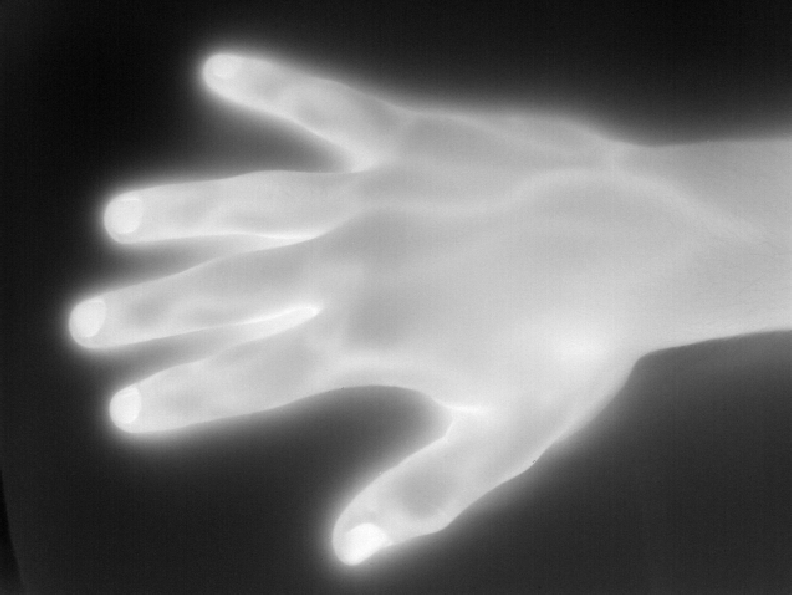
\includegraphics[width=0.6\textwidth]{figures/mat2grayHand}  %<--but is not needed.
	\caption{Image of frame number one for a subject, mat2gray image}
	\label{fig:mat2grayHand}  %<--give the figure a label, so you can reference!
\end{figure}

28 regions on the hand was chosen illustrated on \ref{fig:roiHand} which shows the regions of the hand that is used for the comparison test. The regions gives an pixelintensity value from the mean of the chosen pixel value and the neighbor pixels, so its the mean of nine pixels for each region to get a more generel value for the chosen region.

The regions was chosen to get a full representation of the hand, to see what region that shows the most significant difference in the statiscical test. Also by choosing the regions in the nailfolds which is often used to acess the microcirculatory hemodynamics \cite{martina1998}

\begin{figure}[H]
	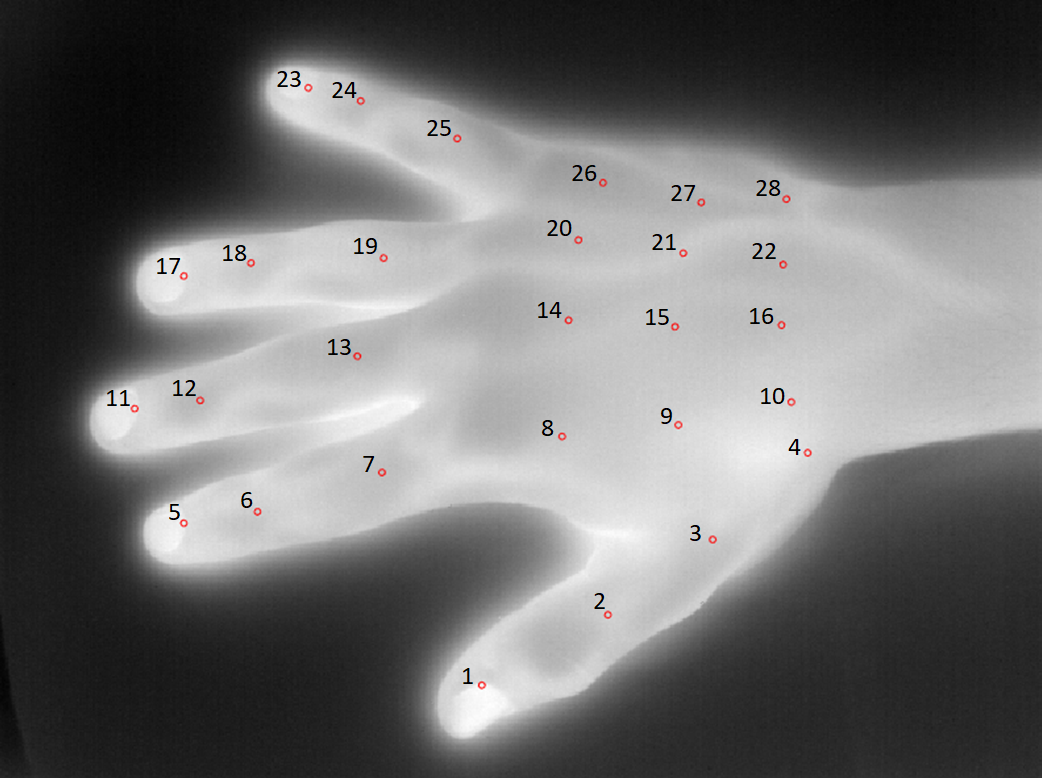
\includegraphics[width=0.6\textwidth]{figures/roiHand}  %<--but is not needed.
	\caption{Image of frame number one for a subject, with regions of interest plottet on 28 areas of the hand}
	\label{fig:roiHand}  %<--give the figure a label, so you can reference!
\end{figure}

The regions is constant for all frames, assuming that the subject was sitting still under the whole measurement. The regions was chosen for each subject by looking at the first frame and finding the coordinates of the center pixel
% The tex should be seen on as fast written worksheets, so some elaboration is needed.